The grey value of each pixel in the detector can be modelled as a random variable, due to the random behaviour of photons being produced, interacting with the test sample and the scintillator in the detector. By modelling using a random variable, the uncertainty can be quantified and considered when conducting inference about any detected defects.

The compound Poisson distribution is studied here because of the compound Poission-like behaviour from the detection of photons \citep{whiting2002signal, elbakri2003efficient, whiting2006properties}. It is defined by defining a latent variable $Y\sim\poisson(\lambda)$ with probability mass function (p.m.f.) $\prob(Y=y)=\euler^{-\lambda}\frac{\lambda^y}{y!}$ for $y=0,1,2,\dotsc$, where $\lambda>0$ is the Poisson rate parameter. Let $U_i$ be some independent and identically distributed (i.i.d.) latent random variables with probability density function (p.d.f.) $p_U(u)$ for $i=1,2,3,\dotsc$. Let $X$ be a compound Poisson random variable where
\begin{equation}
  X|Y = \sum_{i=1}^{Y}U_i \ .
  \label{eq:compoundPoisson_X|Y}
\end{equation}
The p.d.f.~of $X$ can be obtained by marginalising the joint p.d.f.
\begin{equation}
  p_X(x)=\sum_{y=0}^\infty p_{X|Y}(x|y)\prob(Y=y) \quad\text{for }x\geqslant 0
  \ .
\end{equation}
It should be noted that $X=0$ if and only if $Y=0$ and this happens with probability $\prob(Y=0)=\euler^{-\lambda}$. This implies that $X$ has probability mass at zero and probability density for positive numbers which results in the p.d.f.
\begin{equation}
  p_X(x) = 
  \begin{cases}
    \delta(x) \euler^{-\lambda}  & \text{ for } x=0 \\ 
    \sum_{y=1}^\infty p_{X|Y}(x|y)\euler^{-\lambda}\frac{\lambda^y}{y!} \quad\text{for } & \text{ for } x>0
  \end{cases}
\end{equation}
where $\delta(x)$ is the Dirac delta function.

The compound Poisson has applications in, for example, modelling rainfall \citep{revfeim1984initial} and insurance claims \citep{jorgensen1994fitting, smyth2002fitting}.

This chapter starts with a literature review on the compound Poisson distribution, how it is derived from the behaviour of photons, how its likelihood is evaluated and methods for fitting it onto data. A model was proposed for the pixel's grey values and the expectation-maximization (EM) algorithm was implemented to fit the model onto data. It was found that for high photon rate, there were identifiability issues. The chapter is concluded on a discussion on why the EM algorithm failed.

\section{Literature Review}

\subsection{Compound Poisson in X-ray Detection}

In an x-ray tube, photons are emitted as a Poisson process \citep{whiting2006properties, cierniak2011x} and each photon has some random energy due to bremsstrahlung and characteristic radiation \citep{sun2012overview}. This shares similarities to the compound Poisson. Let $Y$ be the number of photons emitted for some time exposure $\tau$, then $Y\sim\poisson(\lambda)$. Each photon is assumed to be i.i.d.~with energy $U_i$ for $i=1,2,3,\dotsc$. $U_i$ has p.d.f.~$p_U(u)$. The random variables discussed here covers all the latent variables in the compound Poisson.

Photons emitted from the x-ray tube undergo attenuation when propagating through the test sample. Assuming no beam hardening, some photons are either absorbed or scattered, making them undetectable. Scattered photons may be detected but it is very rare \citep{cantatore2011introduction}. Attenuated photon energy remains unaffected so attenuation decreases the parameter $\lambda$ and the amount it decreases by depends on the attenuation coefficient of the material and the amount of material the x-ray attenuates. The parameters of the random variable $U_i$ remains unchanged because the energy of each photon remains the same after attenuation, assuming no beam hardening.

When the photons interact with the scintillator in the detector, they are converted into visible light. The visible light photons are then detected and converted into a digital signal. A quantum counter set the digital signal to be linear with to the number of photons detected \citep{whiting2006properties}. Let $X$ be the grey value observed, then
\begin{equation}
X = bY + \epsilon
\end{equation}
where $\epsilon\sim\normal(a,\kappa)$, $b$ and $a$ are some constant and $\kappa$ is the variance of electronic noise. The mean and variance of the grey value are
\begin{equation}
\expectation\left[X\right] = b\lambda + a
\end{equation}
and
\begin{equation}
\variance\left[X\right] = b^2\lambda + \kappa
\end{equation}
respectively. By eliminating $\lambda$
\begin{equation}
\variance\left[X\right] = b\expectation\left[X\right]+\kappa-ab \ ,
\end{equation}
a linear relationship between the variance and expectation of the grey value \citep{ma2012varaince} is obtained.

An energy integrating detector records the grey value as linear to the energy detected \citep{whiting2006properties}. The grey value $X$ is
\begin{equation}
X|Y = \sum_{i=1}^Y U_i + \epsilon \ .
\end{equation}
This is the compound Poisson with Normal noise added to it. The scale factor $b$ is not included as this can be absorbed into $U$. Using the result that $\expectation\left[X\right]=\expectation\expectation\left[X|Y\right]$ and $\variance\left[X\right] = \variance\expectation\left[X|Y\right] + \expectation\variance\left[X|Y\right]$, the mean and variance of the grey value are
\begin{equation}
\expectation\left[X\right] = \lambda\expectation\left[U\right]+a
\end{equation}
and
\begin{equation}
\variance\left[X\right] = \lambda \expectation\left[U^2\right]+\kappa
\end{equation}
respectively. Eliminating $\lambda$ obtains
\begin{equation}
\variance\left[X\right] = \dfrac{\expectation\left[U^2\right]}{\expectation\left[U\right]} \expectation\left[X\right] + \kappa - a\dfrac{\expectation\left[U^2\right]}{\expectation\left[U\right]} \ .
\end{equation}
By assuming no beam hardening, $\expectation\left[U\right]$ and $\expectation\left[U^2\right]$ remains constant, thus there is a linear relationship between the variance and expectation of the grey value \citep{yang2009evaluation}. There are other types of detection schemes \citep{whiting2006properties} but it shall be not be considered here.

Experiments have been done to verify the compound Poisson nature of the detector. This was done by investigating the variance of radiographs of air \citep{hsieh2015compound} and a polyethylene cylinder \citep{yang2009evaluation, yang2010noise} at different voltages and powers. It was found there were two components in the noise, one was signal dependent and comes from the compound Poisson, the other was signal independent and may be electronic noise. The electronic noise can be modelled using a Normal distribution \citep{xu2009electronic}.

\subsection{Moment Generating Function}

Returning back to the compound Poisson with no electronic noise $X|Y = \sum_{i=1}^{Y}U_i$. Let the moment generating function (m.g.f.) of $X$ be $M_X(\theta)=\expectation\left[\euler^{X\theta}\right]$. It can be shown that the m.g.f.~is
\begin{equation}
  M_X(\theta)=
  \exp\left[
    \lambda
    \left(
      M_U(\theta)-1
    \right)
  \right]
\end{equation}
\citep{gatto2010saddlepoint}. The derivation is shown in Appendix \ref{chapter:appendix_compoundPoissonMgf}. Moments of $X$ can be obtained from the m.g.f.~by differentiating it and setting $\theta$ to zero. In other words, $\expectation[X^r]=M_X^{(r)}(0)$. Then it can be shown that
\begin{align}
  \expectation\left[X\right]&=\lambda\expectation\left[U\right]
  \\
  \variance\left[X\right] &= \lambda\expectation\left[U^2\right]
  \\
  \expectation\left[(X-\expectation[X])^3\right] &=\lambda\expectation\left[U^3\right]
\end{align}
which agrees with the expectation and variance results in the previous section. The derivation is shown in Appendix \ref{chapter:appendix_compoundPoissonMgf}.

\subsection{Compound Poisson-Gamma}
\label{chapter:compoundPoisson_compoundPoissonGamma}
A special case of the compound Poisson is when $U\sim\gammaDist\left(\alpha,\beta\right)$ where $\alpha>0$ is the gamma shape parameter and $\beta>0$ is the gamma rate parameter. This was used for example in \cite{xu2009electronic}. This is known as the compound Poisson-gamma distribution. This is denoted by $X\sim\CPoisson(\lambda,\alpha,\beta)$ and has p.d.f.
\begin{equation}
  p_X(x) = 
  \begin{cases}
    \delta(x) \euler^{-\lambda} & \text{ for } x=0 \\ 
    \displaystyle\sum_{y=1}^{\infty}\dfrac{\beta^{y\alpha}}{\Gamma(y\alpha)}x^{y\alpha-1}\euler^{-\beta x}\euler^{-\lambda}\frac{\lambda^y}{y!} & \text{ for } x>0
  \end{cases}
  \ .
  \label{eq:compoundPoisson_pdf}
\end{equation}
Recall that $X|Y=\sum_{i=1}^YU_i$ which involves a sum of gamma random variables. It can be shown that
\begin{equation}
  X|Y\sim\gammaDist\left(Y\alpha,\beta\right).
\end{equation}

The m.g.f.~of $U$ is $M_U(\theta) = \left(\dfrac{\beta}{\beta-\theta}\right)^\alpha$, then the m.g.f.~of $X$ is
\begin{equation}
  M_X(\theta)=\exp\left[\lambda\left(\left(\frac{\beta}{\beta-\theta}\right)^{\alpha}-1\right)\right]
\end{equation}
and moments can be obtained from it such as
\begin{equation}
  \expectation\left[X\right]=\frac{\alpha\lambda}{\beta}
\end{equation}
\begin{equation}
  \variance\left[X\right]=\frac{\alpha(\alpha+1)\lambda}{\beta^2}
  \label{eq:compoundPoisson_variance}
\end{equation}
and
\begin{equation}
  \expectation\left[(X-\expectation[X])^3\right] = \frac{\alpha(\alpha+1)(\alpha+2)\lambda}{\beta^3}
  \ .
\end{equation}

\subsection{Generalised Linear Model}

It can be shown that the compound Poisson-gamma distribution is in the exponential family for fixed $\alpha$ \citep{jorgensen1987exponential}. To show this, it is useful to parametrise the compound Poisson-gamma distribution using the following:
\begin{equation}
  p=\frac{2+\alpha}{1+\alpha}
  \ ,
\end{equation}
\begin{equation}
  \mu=\frac{\lambda\alpha}{\beta}
  \ ,
\end{equation}
\begin{equation}
  \phi = \frac{\alpha+1}{\beta^{2-p}(\lambda\alpha)^{p-1}}
  \ .
\end{equation}
The parameters $p$, $\mu$ and $\phi$ are called the index, mean and dispersion parameters respectively. The parameters take the values of $1<p<2$, $\mu>0$ and $\phi>0$. After parametrising, it can be shown that the p.m.f.~at zero is
\begin{equation}
  \prob(X=0) = \exp
  \left[
      -\frac{\mu^{2-p}}{\phi(2-p)}
  \right]
\end{equation}
and the p.d.f.~for $x>0$ is
\begin{equation}
  p_X(x) = 
  \exp\left[
    \frac{1}{\phi}
    \left(
      x\frac{\mu^{1-p}}{1-p}-\frac{\mu^{2-p}}{2-p}
    \right)
  \right]
  \frac{1}{x}
  \sum_{y=1}^{\infty}W_y(x,p,\phi)
\end{equation}
where
\begin{equation}
  W_y = W_y(x,p,\phi)=\frac{x^{y\alpha}}{\phi^{y(1+\alpha)}(p-1)^{y\alpha}(2-p)^yy!\Gamma(y\alpha)}
  \ .
\end{equation}
The derivation is shown in Appendix \ref{chapter:appendix_tweedie}. This is in the form of a generalised linear model \citep{nelder1972generalized, nelder1972generalized_2, mccullagh1984generalized} for fixed $p$ and $\phi$ because the above is in the form of a distribution in the dispersive exponential family.

Parameter estimation for fixed $p$ can be done via the generalised linear model framework and can be extended to include linear mixed models \citep{zhang2013likelihood}. Estimating $p$ is difficult and various methods were discussed by \cite{zhang2013likelihood}. One way is to estimate $\mu$ and $\phi$ on a grid of $p$'s and then select the $p$ which maximises the likelihood \citep{dunn2005series}.

One special property of the compound Poisson-gamma distribution is that it is in the Tweedie dispersion exponential family \citep{jorgensen1987exponential}. It can be shown that it has a special variance mean relationship
\begin{equation}
  \variance[X] = \phi \mu^p
\end{equation}
where $1<p<2$. This is derived in Appendix \ref{chapter:appendix_tweedie}. It should be noted that this relationship is for fixed $p$ and $\phi$. This is different from the linear variance mean relationship found at the start of the chapter which was for fixed $\alpha$ and $\beta$ from assuming no beam hardening.

\subsection{Method of Moments}

The method of moments is a simpler method to estimate the parameters of a compound Poisson-gamma random variable. Suppose $\widehat{\mu}_1$ is an estimator of $\expectation[X]$ and $\widehat{\mu}_j$ is an estimator of $\expectation\left[\left(X-\expectation[X]\right)^j\right]$ for $j=2,3$. Then the estimators
\begin{equation}
  \widehat{\lambda}=\frac{\widehat{\mu}_1^2\widehat{\mu}_2}{2\widehat{\mu}_2^2-\widehat{\mu}_1\widehat{\mu}_3}
\end{equation}
\begin{equation}
  \widehat{\alpha}=\frac{2\widehat{\mu}_2^2-\widehat{\mu}_1\widehat{\mu}_3}{\widehat{\mu}_1\widehat{\mu}_3-\widehat{\mu}_2^2}
\end{equation}
\begin{equation}
  \widehat{\beta}=\frac{\widehat{\mu}_1\widehat{\mu}_2}{\widehat{\mu}_1\widehat{\mu}_3-\widehat{\mu}_2^2}
\end{equation}
are method of moments estimators of $\lambda$, $\alpha$ and $\beta$ respectively \citep{withers2011compound}, this is shown in Appendix \ref{chapter:appendix_methodofmoments} These estimators suffer because estimation is not done through the sufficient statistics and can be negative, this is a problem because the parameters do not take non-positive values.

\subsection{Normal Approximation}

The evaluation of the density of a compound Poisson-gamma distribution is useful so that the likelihood can be obtained. The likelihood then can be used to find, for example, maximum likelihood estimators. A problem occurs when dealing with the infinite sum in the p.d.f.~because it cannot be simplified. There are a number of approximations or computational methods to evaluate the p.d.f.~such as Fourier inverting the characteristic function \citep{dunn2008evaluation}, using the saddlepoint approximation \citep{daniels1954saddlepoint} or cleverly sum over certain terms in the infinite sum \citep{dunn2005series}. Monte Carlo methods can be used to evaluate the p.d.f.~by simulating compound Poisson-gamma random variables.

The m.g.f.~provides a starting point to what limiting distributions the compound Poisson-gamma distribution converges to for large parameters. These limiting distributions can be used to approximate the p.d.f.~of the compound Poisson-gamma distribution.

It can be shown for large $\lambda$, the Normal approximation \citep{shevtsova2014on} is
\begin{equation}
  X\sim\normal\left(\frac{\lambda\alpha}{\beta},\frac{\lambda\alpha(\alpha+1)}{\beta^2}\right) \ .
\end{equation}
The solution is shown in Appendix \ref{chapter:appendix_normalApproximation}.

\subsection{Saddlepoint Approximation}

The saddlepoint approximation \citep{daniels1954saddlepoint} gives an approximate solution to inverting the Laplace transformation or the m.g.f.~giving the p.d.f.~and has been used in XCT \citep{elbakri2003statistical, elbakri2003efficient}. Inverting the Fourier transformation of the characteristic function also gives the p.d.f.~using computational methods \citep{dunn2008evaluation}. The saddlepoint approximation will be studied here.

For a given m.g.f.~$M_X(\theta)$, the saddlepoint approximation \citep{daniels1954saddlepoint, butler2007saddlepoint} finds an approximate p.d.f.~$p_X(x)$. The saddlepoint approximation is given as
\begin{equation}
  p_X(x)\approx\left(2\pi K_X''(s)\right)^{-1/2}\exp\left[K_X(s)-sx\right]
  \label{eq:saddlePoint:generalSaddlePoint}
\end{equation}
where $K_X(\theta) = \ln\left(M_X(\theta)\right)$, and $s=s(x)$ is the solution to the saddle point equation $K_X'(s)=x$.

For the compound Poisson-gamma distribution, the saddle point approximation \citep{jensen1991saddlepoint} is given as 
\begin{multline}
  p_X(x)\approx
  \frac{\left(\lambda\alpha\beta^\alpha\right)^{\frac{1}{2(\alpha+1)}}\euler^{-\lambda}}{\sqrt{2\pi(\alpha+1)}}x^{-\frac{\alpha+2}{2(\alpha+1)}}
  \euler^{-x\beta}
  \exp\left[x^{\frac{\alpha}{\alpha+1}}
    \frac{(\lambda\beta^\alpha)^{\frac{1}{\alpha+1}}(\alpha+1)}{\alpha^{\frac{\alpha}{\alpha+1}}}
  \right]
  \\
  \text{for }x>0
  \label{eq:saddle_point_approx}
\end{multline}
with the derivation shown in Appendix \ref{chapter:appendix_saddlepoint}. The approximation is not well defined for $x=0$.

The integral of the density approximation over the support may not equal to one, it can be numerically re-normalised if necessary. Thus it may be more sensible to write the approximation up to a constant
\begin{equation}
  p_X(x)\propto x^{-\frac{\alpha+2}{2(\alpha+1)}}\euler^{-x\beta}
  \exp\left[
    x^{\frac{\alpha}{\alpha+1}}
    \frac{
      (\lambda\beta^\alpha)^{\frac{1}{\alpha+1}}(\alpha+1)
    }
    {
      \alpha^{\frac{\alpha}{\alpha+1}}
    }
  \right]
  \ .
\end{equation}

\subsection{Series Evaluation}

The infinite sum, $\sum_{y=1}^\infty W_y$, can be computationally summed in a clever way in order to evaluate the p.d.f. This was done by summing only large terms in the sum and ignore small terms \citep{dunn2005series}. \cite{dunn2005series} approximated the sum by truncation
\begin{equation}
  \sum_{y=1}^\infty W_y \approx \sum_{y=y_\text{l}}^{y_\text{u}}W_y
\end{equation}
where $y_\text{l}<y_{\text{max}}<y_\text{u}$ and $y_{\text{max}}$ is the value of $y$ which maximises $W_y$. \cite{dunn2005series} used Stirling's approximation to find that
\begin{equation}
  y_{\text{max}} \approx \frac{x^{2-p}}{\phi(2-p)}
\end{equation}
by treating $W_y$ as a continuous and differentiable function of $y$. The derivation is shown in Appendix \ref{chapter:appendix_compoundPoissonSeries}. Because values of $y$ should be a positive integer, it would be appropriate to round the solution to $y_\text{max}$ accordingly
\begin{equation}
  y_{\text{max}} = \text{max}\left[
    1,\text{round}\left(\frac{x^{2-p}}{\phi(2-p)}\right)
  \right]
  \ .
\end{equation}

$y_\text{l}$ and $y_\text{u}$ can be chosen such that $W_{y_\text{l}}$ and $W_{y_\text{u}}$ are less than $\epsilon W_{y_\text{max}}$ where $\epsilon$ is some small constant, for example $\epsilon=\euler^{-37}$ will be better than machine precision in 64 bits \citep{dunn2005series}. To prevent overflow problems, it is advised to calculate each term in the summation in log scale \citep{dunn2005series} by using the following equation
\begin{equation}
  \ln\left[
    \sum_{y=y_\text{l}}^{y_\text{u}}W_y
  \right]
  = 
  \ln\left(
    W_{y_\text{max}}
  \right)
  +\ln\sum_{y=y_\text{l}}^{y_\text{u}}
  \exp\left[
    \ln\left(W_y\right)-\ln\left(W_{y_\text{max}}\right)
  \right]
  \ .
\end{equation}

\section{Simulation Studies on Density Evaluation}

Simulations of a compound Poisson-gamma random variable were conducted with the aim to compare how well these density evaluations methods perform. This was done by comparing the evaluated densities with the histogram of simulations and a Q-Q plot. The following compound Poisson-gamma distributions were used in the simulations to capture the variety in the compound Poisson-gamma family: $\CPoisson(1,1,1)$, $\CPoisson(1,100,1)$, $\CPoisson(10,1,1)$, $\CPoisson(100,100,1)$. Varying $\beta$ is not interesting here as this only scales the random variable.

There were a few technical problems with the histogram because the compound Poisson has probability mass at zero and probability density for positive numbers. To correctly represent the empirical distribution of a compound Poisson random variable, a bar chart was used to show the frequency of a zero and a histogram to show the frequency density of positive numbers. However, the Normal approximation and the saddlepoint approximation does not have mass support at zero. Therefore, to compare these approximate densities to the empirical distribution fairly, a histogram containing both zero and positive samples was used when appropriate.

The evaluation of the p.d.f.~using the saddlepoint approximate required a bit of caution to avoid over/underflow problems. Suppose realizations of $X$ were simulated $\left\{x_1,x_2,x_3,\dotsc,x_n\right\}$. The saddlepoint approximation was computed up to a constant using
\begin{equation}
  p_X(x) \propto
  \exp\left[
    -\frac{\alpha+2}{2(\alpha+1)}
    \ln(x)
    -x\beta
    +\left(
    \frac{x\beta}{\alpha}
    \right)^{\frac{\alpha}{\alpha+1}}\lambda^{\frac{1}{\alpha+1}}(\alpha+1) - k
  \right]
\end{equation}
for 10\,000 equally spaced points from and including the minimum non-zero simulated value to the maximum simulated value. $k$ is some constant which was chosen to be
\begin{equation}
  k =
  \max_{i\in\left\{1,2,3,\dotsc,n\right\}}
  \left[
    -\frac{\alpha+2}{2(\alpha+1)}
    \ln(x_i)
    -x_i\beta
    +\left(
      \frac{x_i\beta}{\alpha}
    \right)^{\frac{\alpha}{\alpha+1}}\lambda^{\frac{1}{\alpha+1}}(\alpha+1)
  \right]
  \ .
\end{equation}
The density was then was normalised by numerically integrating it using the trapezium rule using the 10\,000 evaluated points.

A Q-Q plot is a plot which compares the empirical quantiles with the theoretical quantiles. Let
\begin{equation}
  F_X(x) = \prob(X\leqslant x)
\end{equation}
and
\begin{equation}
  \widehat{F}_X(x) = \frac{1}{n}\cdot\text{max}
  \left[
    \left(\sum_{i=1}^n\mathbb{I}(x_i\leqslant x)\right)-0.5,0
  \right]
  \ ,
\end{equation}
then a Q-Q plot is a parametric plot which plots $\widehat{F}_X^{-1}(p)$ against $F_X^{-1}(p)$ for $p=\frac{0.5}{n},\frac{1.5}{n},\frac{2.5}{n},\dotsc,\frac{n-0.5}{n}$. If $F_X(x)$ and $\widehat{F}_X(x)$ are similar, a Q-Q plot should be a straight line with gradient 1, intercepting the origin. For the exact method and the saddlepoint approximation, $F_X(x)$ was found numerically by evaluating the p.d.f.~at $10\,000$ equally spaced points from and including the minimum to the maximum of the simulated samples, and then summing the required trapeziums. Because the saddlepoint approximation does not support zero, the numerical integration cannot start at zero. $\widehat{F}_X^{-1}(p)$ was then calculated by interpolation.

When plotting the probability of obtaining a zero or the p.d.f.~for positive values, confidence intervals were plotted as well. Consider a bin in a histogram, the confidence intervals were obtained by assuming that the frequency in a bin $\sim\poisson(\text{p.d.f.~evaluated at the bin}\times 1\,000 \times \text{bin width})$.

For low $\lambda$ (Figures \ref{fig:compoundPoisson_histogram_1_1_1}to \ref{fig:compoundPoisson_histogram_approx_1_100_1}) there is a chance of simulating zeros. For $\lambda = 1$, the Normal approximation failed to capture the probability mass at zero because the Normal distribution is symmetric and support negative values. The saddlepoint approximation did capture the probability mass at zero as shown by an increase in probability density towards zero. For $\CPoisson(1,100,1)$ in Figure \ref{fig:compoundPoisson_histogram_approx_1_100_1}, the compound Poisson-gamma p.d.f.~contains multiple peaks and the saddlepoint approximation was not flexible enough to capture them. In Figure \ref{fig:compoundPoisson_histogram_1_100_1}, the Q-Q plot for the exact method was quite sensitive at the tails of each peak, perhaps there were a few inaccuracies in the exact evaluation of the p.d.f.~or in the calculation of the numerical calculation of the c.d.f.~and its inversion.

As $\lambda$ increased, in Figures \ref{fig:compoundPoisson_histogram_10_1_1} and \ref{fig:compoundPoisson_histogram_100_1_1}, all 3 density evaluation methods performed quite well. For $\CPoisson(10,1,1)$ in Figure \ref{fig:compoundPoisson_histogram_10_1_1}, the Normal approximation did not quite capture the skewness. In Figure \ref{fig:compoundPoisson_histogram_100_1_1}, $\lambda$ was high enough where the compound-Poisson distribution starts to converge to a Normal distribution. All methods performed well in this realm.

\begin{figure}
  \centering
    \centerline{
    \begin{subfigure}[b]{\mainSize}
        \includegraphics[width=\textwidth]{../figures/compoundpoisson/cpHistogram_CompoundPoissonlambda1alpha1beta1.eps}
        \caption{Left: Observed and expected frequency of a zero. Right: Histogram and p.d.f.~of non-zero values.}
    \end{subfigure}
    }
    \vspace{2em}
    \centerline{
    \begin{subfigure}[b]{\subSize}
        \includegraphics[width=\textwidth]{../figures/compoundpoisson/cpHistogram_qq_CompoundPoissonlambda1alpha1beta1.eps}
        \caption{Q-Q plot}
    \end{subfigure}
    }
    \caption{1\,000 $\CPoisson(1,1,1)$ random variables were simulated and its empirical distribution is compared to the p.d.f.~evaluated using the exact method. In a), the dotted red line shows the 68\% confidence interval of the expected frequency or frequency density.}
    \label{fig:compoundPoisson_histogram_1_1_1}
\end{figure}

\begin{figure}
  \centering
    \centerline{
    \begin{subfigure}[b]{\mainSize}
        \includegraphics[width=\textwidth]{../figures/compoundpoisson/cpHistogram_CompoundPoissonlambda1alpha100beta1.eps}
        \caption{Left: Observed and expected frequency of a zero. Right: Histogram and p.d.f.~of non-zero values.}
    \end{subfigure}
    }
    \vspace{2em}
    \centerline{
    \begin{subfigure}[b]{\subSize}
        \includegraphics[width=\textwidth]{../figures/compoundpoisson/cpHistogram_qq_CompoundPoissonlambda1alpha100beta1.eps}
        \caption{Q-Q plot}
    \end{subfigure}
    }
    \caption{1\,000 $\CPoisson(1,100,1)$ random variables were simulated and its empirical distribution is compared to the p.d.f.~evaluated using the exact method. In a), the dotted red line shows the 68\% confidence interval of the expected frequency or frequency density.}
    \label{fig:compoundPoisson_histogram_1_100_1}
\end{figure}

\begin{figure}
  \centering
    \centerline{
    \begin{subfigure}[b]{\subSize}
        \includegraphics[width=\textwidth]{../figures/compoundpoisson/cpHistogram_CompoundPoissonNormlambda1alpha1beta1.eps}
        \caption{Histogram - Normal approx.}
    \end{subfigure}
    \begin{subfigure}[b]{\subSize}
        \includegraphics[width=\textwidth]{../figures/compoundpoisson/cpHistogram_qq_CompoundPoissonNormlambda1alpha1beta1.eps}
        \caption{Q-Q plot - Normal approx.}
    \end{subfigure}
    }
    \vspace{1em}
    \centerline{
    \begin{subfigure}[b]{\subSize}
        \includegraphics[width=\textwidth]{../figures/compoundpoisson/cpHistogram_CompoundPoissonSaddlelambda1alpha1beta1.eps}
        \caption{Histogram - Saddlepoint approx.}
    \end{subfigure}
    \begin{subfigure}[b]{\subSize}
        \includegraphics[width=\textwidth]{../figures/compoundpoisson/cpHistogram_qq_CompoundPoissonSaddlelambda1alpha1beta1.eps}
        \caption{Q-Q plot - Saddlepoint approx.}
    \end{subfigure}
    }
    \caption{1\,000 $\CPoisson(1,1,1)$ random variables were simulated and its empirical distribution is compared to the approximate p.d.f. On the left, the dotted red line shows the 68\% confidence interval of the expected frequency density.}
    \label{fig:compoundPoisson_histogram_approx_1_1_1}
\end{figure}

\begin{figure}
  \centering
    \centerline{
    \begin{subfigure}[b]{\subSize}
        \includegraphics[width=\textwidth]{../figures/compoundpoisson/cpHistogram_CompoundPoissonNormlambda1alpha100beta1.eps}
        \caption{Histogram - Normal approx.}
    \end{subfigure}
    \begin{subfigure}[b]{\subSize}
        \includegraphics[width=\textwidth]{../figures/compoundpoisson/cpHistogram_qq_CompoundPoissonNormlambda1alpha100beta1.eps}
        \caption{Q-Q plot - Normal approx.}
    \end{subfigure}
    }
    \vspace{1em}
    \centerline{
    \begin{subfigure}[b]{\subSize}
        \includegraphics[width=\textwidth]{../figures/compoundpoisson/cpHistogram_CompoundPoissonSaddlelambda1alpha100beta1.eps}
        \caption{Histogram - Saddlepoint approx.}
    \end{subfigure}
    \begin{subfigure}[b]{\subSize}
        \includegraphics[width=\textwidth]{../figures/compoundpoisson/cpHistogram_qq_CompoundPoissonSaddlelambda1alpha100beta1.eps}
        \caption{Q-Q plot - Saddlepoint approx.}
    \end{subfigure}
    }
    \caption{1\,000 $\CPoisson(1,100,1)$ random variables were simulated and its empirical distribution is compared to the approximate p.d.f. On the left, the dotted red line shows the 68\% confidence interval of the expected frequency density.}
    \label{fig:compoundPoisson_histogram_approx_1_100_1}
\end{figure}

\begin{figure}
  \centering
    \centerline{
    \begin{subfigure}[b]{\subSize}
        \includegraphics[width=\textwidth]{../figures/compoundpoisson/cpHistogram_CompoundPoissonlambda10alpha1beta1.eps}
        \caption{Histogram - Exact method}
    \end{subfigure}
    \begin{subfigure}[b]{\subSize}
        \includegraphics[width=\textwidth]{../figures/compoundpoisson/cpHistogram_qq_CompoundPoissonlambda10alpha1beta1.eps}
        \caption{Q-Q plot - Exact method}
    \end{subfigure}
    }
    \centerline{
    \begin{subfigure}[b]{\subSize}
        \includegraphics[width=\textwidth]{../figures/compoundpoisson/cpHistogram_CompoundPoissonNormlambda10alpha1beta1.eps}
        \caption{Histogram - Normal approx.}
    \end{subfigure}
    \begin{subfigure}[b]{\subSize}
        \includegraphics[width=\textwidth]{../figures/compoundpoisson/cpHistogram_qq_CompoundPoissonNormlambda10alpha1beta1.eps}
        \caption{Q-Q plot - Normal approx.}
    \end{subfigure}
    }
    \centerline{
    \begin{subfigure}[b]{\subSize}
        \includegraphics[width=\textwidth]{../figures/compoundpoisson/cpHistogram_CompoundPoissonSaddlelambda10alpha1beta1.eps}
        \caption{Histogram - Saddlepoint approx.}
    \end{subfigure}
    \begin{subfigure}[b]{\subSize}
        \includegraphics[width=\textwidth]{../figures/compoundpoisson/cpHistogram_qq_CompoundPoissonSaddlelambda10alpha1beta1.eps}
        \caption{Q-Q plot - Saddlepoint approx.}
    \end{subfigure}
    }
    \caption{1\,000 $\CPoisson(10,1,1)$ random variables were simulated and its empirical distribution is compared to the p.d.f. On the left, the dotted red line shows the 68\% confidence interval of the expected frequency density.}
    \label{fig:compoundPoisson_histogram_10_1_1}
\end{figure}

\begin{figure}
  \centering
    \centerline{
    \begin{subfigure}[b]{\subSize}
        \includegraphics[width=\textwidth]{../figures/compoundpoisson/cpHistogram_CompoundPoissonlambda100alpha100beta1.eps}
        \caption{Histogram - Exact method}
    \end{subfigure}
    \begin{subfigure}[b]{\subSize}
        \includegraphics[width=\textwidth]{../figures/compoundpoisson/cpHistogram_qq_CompoundPoissonlambda100alpha100beta1.eps}
        \caption{Q-Q plot - Exact method}
    \end{subfigure}
    }
    \centerline{
    \begin{subfigure}[b]{\subSize}
        \includegraphics[width=\textwidth]{../figures/compoundpoisson/cpHistogram_CompoundPoissonNormlambda100alpha100beta1.eps}
        \caption{Histogram - Normal approx.}
    \end{subfigure}
    \begin{subfigure}[b]{\subSize}
        \includegraphics[width=\textwidth]{../figures/compoundpoisson/cpHistogram_qq_CompoundPoissonNormlambda100alpha100beta1.eps}
        \caption{Q-Q plot - Normal approx.}
    \end{subfigure}
    }
    \centerline{
    \begin{subfigure}[b]{\subSize}
        \includegraphics[width=\textwidth]{../figures/compoundpoisson/cpHistogram_CompoundPoissonSaddlelambda100alpha100beta1.eps}
        \caption{Histogram - Saddlepoint approx.}
    \end{subfigure}
    \begin{subfigure}[b]{\subSize}
        \includegraphics[width=\textwidth]{../figures/compoundpoisson/cpHistogram_qq_CompoundPoissonSaddlelambda100alpha100beta1.eps}
        \caption{Q-Q plot - Saddlepoint approx.}
    \end{subfigure}
    }
    \caption{1\,000 $\CPoisson(100,100,1)$ random variables were simulated and its empirical distribution is compared to the p.d.f. On the left, the dotted red line shows the 68\% confidence interval of the expected frequency density.}
    \label{fig:compoundPoisson_histogram_100_1_1}
\end{figure}

\section{Proposed Model}

The compound Poisson-gamma distribution can be used to model the grey values of each pixel in a projection. Suppose a projection has $m$ pixels and $n$ replicate projections were obtained. Let $X_{i,j}$ and $Y_{i,j}$ be the grey value and photon count, respectively, of the $i$th pixel in the $j$th replicate projection.

By assuming no beam hardening, the distribution of the photon energy does not change with attenuation. As a result all pixels will detect photons with identical energy distributions thus $\alpha$ and $\beta$ are the same for all pixels. Attenuation does affect the photon count, the more material a photon has to attenuate, the lower the number of detectable photons. The amount of attenuation depends on the specific path from the source to a pixel in a detector, so $\lambda_i$ varies from pixel to pixel. Electronic Normal noise $\epsilon_{i,j}\sim\normal(a,\kappa)$ may be added as well.

\begin{figure}
  \centering
  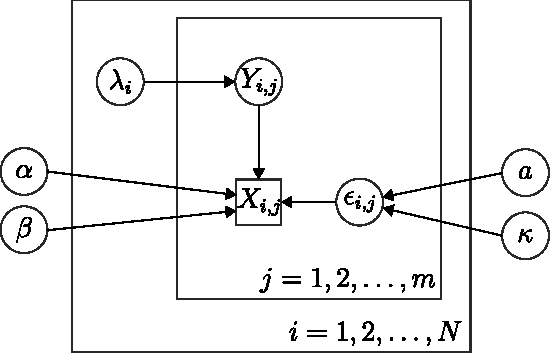
\includegraphics[width=0.6\textwidth]{../figures/compoundpoisson/graphicalModel.pdf}
  \caption{Graphical model of the grey value $X_{i,j}$ for each of the $m$ pixels in the $n$ replicate projections. $Y_{i,j}\sim\poisson(\lambda_i)$ is the photon count. The grey value has a compound Poisson gamma element $X_{i,j}|Y_{i,j}\sim\gammaDist(Y_{i,j}\alpha,\beta)$ and can be extended by adding electronic noise $\epsilon_{i,j}\sim\normal(a,\kappa)$.}
  \label{fig:compoundPoisson_graphicalModel}
\end{figure}

The graphical model in Figure \ref{fig:compoundPoisson_graphicalModel} illustrates how all of these variables link together. $a$ and $\kappa$ are unknown parameters but can be estimated beforehand from replicate black images. Care must be taken to use the replicate black images for either shading correction or for estimating $a$ and $\kappa$ to avoid using the data twice. The energy of each photon $U\sim\gammaDist(\alpha,\beta)$ was omitted in the graphical model because the conditional distribution $X|Y\sim\gammaDist(Y\alpha,\beta)$ encapsulates each detected photon energy already.

The model may be simplified by omitting the electronic noise, this can be done by setting $a=0$ and $\kappa=0$. The number of pixels can be set to $m=1$ as well. Parameter estimation can be done using gradient methods because the likelihood of the compound Poisson can be evaluated \citep{dunn2005series}. However, the EM algorithm is faster and the model is well set up for it.

\section{EM Algorithm}

The EM algorithm \citep{dempster1977maximum} is proposed as a method to estimate the parameters of a $X\sim\CPoisson(\lambda,\alpha,\beta)$ random variable given a sample of measurements of it $\left\{x_1,x_2,x_3,\dotsc,x_n\right\}$. The use of the EM algorithm for the compound Poisson in XCT has been studied in \cite{elbakri2003statistical, xie2008x, xu2009electronic}.

Let $\widehat{\lambda}$, $\widehat{\alpha}$ and $\widehat{\beta}$ be estimators of $\lambda$, $\alpha$ and $\beta$ respectively. The log likelihood is defined to be
\begin{equation*}
  \ln L(\lambda,\alpha,\beta;X) = \sum_{i=1}^n
  \left[
    \mathbb{I}(x_i=0)\ln \prob(X=x_i)
    +\mathbb{I}(x_i>0)\ln p_X(x_i)
  \right]
\end{equation*}
and using the results in Appendix \ref{chapter:appendix_tweedie}
\begin{equation}
  \ln L(\lambda,\alpha,\beta;X) =
    \sum_{i=1}^n
    \left[
      -\mathbb{I}(x_i=0)\lambda
      \vphantom{\sum_i^i}
    \right.
    {}\\
    \left.
      +\mathbb{I}(x_i>0)\left(
      -\beta x_i-\lambda-\ln x +\ln\sum_{y=1}^\infty W_y
      \right)
    \right] \ .
\end{equation}
Maximum likelihood estimators are values of $\lambda$, $\alpha$ and $\beta$ which jointly maximises the log likelihood.

The EM algorithm \citep{dempster1977maximum} instead treats $Y\sim\poisson(\lambda)$ as a latent variable. Let $\left\{Y_1,Y_2,Y_3,\dotsc, Y_n\right\}$ be realizations of $Y$ and $\left\{x_1,x_2,x_3,\dotsc, x_n\right\}$ be the respective measurements of $X|Y$. Define the joint log likelihood to be
\begin{multline*}
  \ln L(\lambda,\alpha,\beta;X,Y)
  =
  \sum_{i=1}^n
  \left[
    \mathbb{I}(x_i=0)
    \ln
    \prob(Y=0)
  \right.
  \\
  \left.
    +
    \mathbb{I}(x_i>0)
    \ln
    \left[
      p_{X|Y}(x_i|Y_i)\prob(Y=Y_i)
    \right]
  \right]
\end{multline*}
so that
\begin{multline}
  \ln L(\lambda,\alpha,\beta;X,Y)=
  \sum_{i=1}^n
  \left[
    -\mathbb{I}(x_i=0)
    \lambda
  \right.
  \\
  \left.+
    \mathbb{I}(x_i>0)
    \left(
      Y_i\alpha\ln\beta-\ln\Gamma(Y_i\alpha)+(Y_i\alpha-1)\ln x_i - \beta x_i
    \right.
  \right.
  \\
  \left.
    \left.  
      - \lambda + Y_i \ln \lambda - \ln(Y_i!)
    \right)
  \right]
  \ .
\end{multline}
The estimators are found by optimising the joint log likelihood. This is done iteratively by estimating the $Y$s given the $X$s and parameters (E step), followed by estimating the parameters given the $Y$s and $X$s (M step) until some convergence conditions are met.

It will be shown that using some approximations, the E step and M step can be implemented. The Cram\'er-Rao lower bound \citep{rao1945information, cramer1946mathematical} can also be found by using a few approximations. However, simulations showed that these estimators struggle for high $\lambda$.

\subsection{E Step}

In the E step, the realizations of $Y$ are estimate using
\begin{equation}
  y_i =
  \expectation\left[
    Y|X=x_i
  \right]
\end{equation}
for given parameters $\lambda$, $\alpha$ and $\beta$. The conditional expectation is calculated using
\begin{equation}
  y_i = 
  \begin{cases}
    0 & \text{ for } x=0 \\ 
    \dfrac{\sum_{y=1}^\infty y \prob(Y=y|X=x_i)}{\sum_{y=1}^\infty \prob(Y=y|X=x_i)} & \text{ for } x>0
  \end{cases}
\end{equation}
where
\begin{equation*}
  \prob(Y=y|X=x) = \frac{p_{X|Y}(x|y)\prob(Y=y)}{p_X(x)}
  \ .
\end{equation*}
Focussing on the $x>0$ case for now
\begin{equation*}
  \prob(Y=y|X=x) = \frac{1}{p_X(x)}\frac{\beta^{y\alpha}}{\Gamma(y\alpha)}x^{y\alpha-1}\euler^{-\beta x}\frac{\euler^{-\lambda}\lambda^y}{y!}
\end{equation*}
and
\begin{equation}
  \prob(Y=y|X=x) = W_y \frac{\euler^{-\lambda-\beta x}}{x p_X(x)} \ .
\end{equation}
Then the conditional expectation is
\begin{equation}
  y_i = \frac{\sum_{y=1}^\infty y W_y}{\sum_{y=1}^\infty W_y}
  \ .
\end{equation}
As discussed before, the sum in the denominator can be evaluated using the method by \cite{dunn2005series}. A similar method for evaluating the numerator can be obtained by truncating the sum and summing large terms.

Let
\begin{equation}
  W_y^{(r)} = y^r W_y \quad \text{for }r=1,2,3,\dotsc
\end{equation}
so that
\begin{equation}
  y_i = \frac{\sum_{y=1}^\infty W^{(1)}_y}{\sum_{y=1}^\infty W_y} \ .
\end{equation}
Similarly
\begin{equation}
  \zeta_i = \variance[Y|X=x_i] = \frac{\sum_{y=1}^\infty W^{(2)}_y}{\sum_{y=1}^\infty W_y} - \left(y_i\right)^2
  \ .
\end{equation}
The expectation terms, $y_i$ and $\zeta_i$, are evaluated in the M step so that they can be used in the E step. The evaluation can be done by truncating the sum
\begin{equation}
  \sum_{y=1}^\infty W^{(r)}_y \approx \sum_{y=y_\text{l}}^{y_\text{u}} W^{(r)}_y
\end{equation}
where $y_\text{l}<y_\text{max}<y_\text{u}$ and $y_\text{max}$ is the value of $y$ which maximises $W_y^{(r)}$. By expressing $\ln(W^{(r)}_y)$ as
\begin{equation}
  \ln\left(W_y^{(r)}\right)=r\ln(y)+\ln(W_y)
\end{equation}
and then taking the derivative with respect to $y$
\begin{equation}
  \frac{\partial \ln(W_y^{(r)})}{\partial y} = \frac{r}{y } + \frac{\partial \ln(W_y)}{\partial y}
  \ .
\end{equation}
Keep in mind that $y=1,2,3,\dotsc$ so for large $y$, an approximation can be made $r/y\approx 0$ so that
\begin{equation}
  \frac{\partial \ln(W_y^{(r)})}{\partial y} \approx \frac{\partial \ln(W_y)}{\partial y}
  \ .
\end{equation}
Therefore the maximum of $W_y^{(r)}$ is located at $y_\text{max}$ for all $r=0,1,2,\dotsc$. The same method of evaluating $W_y$ can be used to evaluate $W_y^{(r)}$. For a given $r=0,1,2,\dotsc$, the limit of the sum $\sum_{y=y_\text{l}}^{y_\text{u}} W^{(r)}_y$ are chosen such that $W_{y_\text{l}}$ and $W_{y_\text{u}}$ are less than $\epsilon W_{y_\text{max}}^{(r)}$ where $\epsilon$ is some small constant. The limits will be different for different values of $r$.

\subsection{M Step}

In the M step, the conditional expected joint log likelihood is maximised with respect to the parameters $\lambda$, $\alpha$ and $\beta$. The objective function is
\begin{align}
  T(\lambda,\alpha,\beta)&=
  \begin{multlined}[t]
    \sum_{i=1}^n
    \expectation\left[
      -\mathbb{I}(x_i=0)
      \lambda
    \right.
    \\
    \left.+
      \mathbb{I}(x_i>0)
      \left(
        Y_i\alpha\ln\beta-\ln\Gamma(Y_i\alpha)+(Y_i\alpha-1)\ln x_i - \beta x_i
      \right.
    \right.
    \\
    \left.
      \left.  
        - \lambda + Y_i \ln \lambda - \ln(Y_i!)
      \right)
      |X_i=x_i
    \right]
  \end{multlined}
  \nonumber\\
  &\!\begin{multlined}[b]=
    -n\lambda
    \\
    +\sum_{i=1}^n
    \mathbb{I}(x_i>0)
    \left[
      \expectation[Y_i|X_i=x_i]\alpha\ln\beta-\expectation[\ln\Gamma(Y_i\alpha)|X_i=x_i]
    \right.
    {}\\
    \left.
      +\expectation[Y_i|X_i=x_i]\alpha\ln x_i - \beta x_i
      + \expectation[Y_i|X_i=x_i] \ln \lambda
    \right] + c
  \end{multlined}
\end{align}
where $c$ is some constant not dependent on $\lambda$, $\alpha$ or $\beta$.

The conditional expectation $y_i = \expectation[Y_i|X_i=x_i]$ and $\zeta_i = \variance[Y_i|X_i=x_i]$ were calculated beforehand in the E step. The quantity $\expectation[\ln\Gamma(Y_i\alpha)|X_i=x_i]$ can be calculated using the approximation
\begin{equation}
  \expectation[\ln\Gamma(Y_i\alpha)|X_i=x_i] \approx
  \ln\Gamma(\alpha y_i) + \frac{1}{2}\zeta_i\alpha^2\psi'(y_i\alpha)
\end{equation}
where $\psi(n)$ is the digamma function. The objective function is then
\begin{multline}
  T(\lambda,\alpha,\beta)=
  -n\lambda
  +\sum_{i=1}^n
  \mathbb{I}(x_i>0)
  \left[
    y_i\alpha\ln\beta-\ln\Gamma(\alpha y_i) - \frac{1}{2}\zeta_i\alpha^2\psi'(y_i\alpha)
  \right.
  \\
  \left.
    +y_i\alpha\ln x_i - \beta x_i
    + y_i \ln \lambda
    \vphantom{\frac{1}{1}}
  \right]
  + c
  \ .
\end{multline}

Taking the derivative with respect to $\lambda$
\begin{equation}
  \frac{\partial T}{\partial\lambda} = -n + \frac{\sum_{i=1}^ny_i}{\lambda}
\end{equation}
and setting it to zero
\begin{equation}
  \widehat{\lambda} = \frac{\sum_{i=1}^n y_i}{n}
\end{equation}
obtains a M step estimator, and a familiar one, for $\lambda$. Taking the second derivative with respect to $\lambda$
\begin{equation}
  \frac{\partial^2 T}{\partial \lambda^2} = -\frac{\sum_{i=1}^ny_i}{\lambda^2} < 0
\end{equation}
verifies $\widehat{\lambda}$ maximises T. In addition
\begin{equation}
  \frac{\partial^2 T}{\partial \alpha \partial \lambda } = 0
\end{equation}
and
\begin{equation}
  \frac{\partial^2 T}{\partial \beta \partial \lambda } = 0
  \ .
\end{equation}

Maximising $T$ with respect to $\alpha$ and $\beta$ can be done numerically using the Newton-Raphson method since derivatives up to the second order can be obtained. For the first order these are:
\begin{multline}
  \frac{\partial T}{\partial \alpha} =
  \sum_{i=1}^n\mathbb{I}(x_i>0)
  \left[
    y_i\ln\beta -\psi(\alpha y_i)y_i-\zeta_i\alpha\psi'(\alpha y_i)
    \vphantom{\frac{1}{1}}
  \right.
  \\
  \left.
    - \frac{1}{2}\zeta_i\alpha^2\psi''(\alpha y_i)y_i + y_i\ln x_i
  \right]
\end{multline}
and
\begin{equation}
  \frac{\partial T}{\partial \beta} = \sum_{i=1}^n\mathbb{I}(x_i>0)\left[
  \frac{\alpha y_i}{\beta}-x_i
  \right]
  \ .
\end{equation}
The second orders are:
\begin{equation}
  \frac{\partial^2 T}{\partial \alpha \partial \beta} =
  \sum_{i=1}^n \mathbb{I}(x_i>0)\left[\frac{y_i}{\beta}\right]
  \ ,
  \label{eq:compoundPoisson:d2tdadb}
\end{equation}
\begin{equation}
  \frac{\partial^2 T}{\partial \beta^2} = \sum_{i=1}^n\mathbb{I}(x_i>0)\left[-\frac{\alpha y_i}{\beta^2}
  \right]
  \label{eq:compoundPoisson:d2td2b}
\end{equation}
and
\begin{multline*}
  \frac{\partial^2 T}{\partial \alpha^2} = 
  \sum_{i=1}^n\mathbb{I}(x_i>0)
  \left[
    -y_i^2\psi'(\alpha y_i) - \zeta_i\psi'(\alpha y_i) - \zeta_i\alpha y_i\psi''(\alpha y_i)
    \vphantom{\frac{1}{2}}\right.\\\left. 
    - \zeta_i\alpha\psi''(\alpha y_i)y_i
    -\frac{1}{2}\zeta_i\alpha^2\psi'''(\alpha y_i)y_i^2
  \right]
\end{multline*}
simplifying to
\begin{multline}
  \frac{\partial^2 T}{\partial \alpha^2} = 
  \sum_{i=1}^n\mathbb{I}(x_i>0)
  \left[
    -(y_i^2+\zeta_i)\psi'(\alpha y_i) - 2\zeta_i\alpha y_i\psi''(\alpha y_i)
    \vphantom{\frac{1}{2}}
  \right.
  \\
  \left.  
    -\frac{1}{2}\zeta_i\alpha^2y_i^2\psi'''(\alpha y_i)
  \right] \ .
  \label{eq:compoundPoisson:d2td2a}
\end{multline}

All the derivatives can be used in the Newton-Raphson iterative update to update the estimators $\widehat{\alpha}$ and $\widehat{\beta}$. The update is
\begin{equation}
  \begin{pmatrix}
    \widehat{\alpha} \\ \widehat{\beta}
  \end{pmatrix}
  \leftarrow
  \begin{pmatrix}
    \widehat{\alpha} \\ \widehat{\beta}
  \end{pmatrix}
  -
  \left[
    \nabla_{\alpha,\beta}\nabla_{\alpha,\beta}\T \left. T \right |_{\alpha = \widehat{\alpha}, \beta=\widehat{\beta}}
  \right]^{-1}
  \left[
    \nabla_{\alpha,\beta} \left. T \right |_{\alpha = \widehat{\alpha}, \beta=\widehat{\beta}}
  \right]
\end{equation}
where
\begin{equation}
  \nabla_{\alpha,\beta}=
  \begin{pmatrix}
    {\partial}/{\partial \alpha}
    \\
    {\partial}/{\partial \beta}
  \end{pmatrix}
  \ .
\end{equation}
Since increasing $T$ is sufficient for the EM algorithm \citep{dempster1977maximum}, one step of the Newton-Raphson iterative update was chosen in the M step to avoid implementing a convergence condition.

\subsection{Estimation Error}

The variance of the M step estimators can be obtained by using the Cram\'er-Rao lower bound \citep{rao1945information, cramer1946mathematical} from the Fisher's information matrix defined as
\begin{equation}
  \matr{I} = -\expectation\left[
    \nabla_{\lambda,\alpha,\beta}\nabla_{\lambda,\alpha,\beta}\T \ln L(\lambda,\alpha,\beta;X,Y)
  \right]
\end{equation}
where
\begin{equation}
  \nabla_{\lambda, \alpha,\beta}=
  \begin{pmatrix}
    {\partial}/{\partial \lambda}
    \\
    {\partial}/{\partial \alpha}
    \\
    {\partial}/{\partial \beta}
  \end{pmatrix}
  \ .
\end{equation}
The calculation is similar to the derivatives of $T$ using the same approximations. Using the fact that $\expectation[Y]=\lambda$ and another approximation $\expectation\left[\psi^{(r)}(\alpha Y)\right]\approx\psi^{(r)}(\alpha \lambda)$, then
\begin{equation}
  \matr{I}=
  \begin{pmatrix}
    \dfrac{n}{\lambda} & 0 & 0 \\
    0 & (\lambda^2+\lambda)\psi'(\alpha\lambda)+2\alpha\lambda^2\psi''(\alpha\lambda)+\frac{1}{2}\alpha^2\lambda^3\psi'''(\alpha\lambda) & -\dfrac{n\lambda}{\beta}\\
    0 & -\dfrac{n\lambda}{\beta} & \dfrac{n\alpha\lambda}{\beta^2}
  \end{pmatrix}
  \ .
\end{equation}
The Cram\'er-Rao lower bound is then
\begin{equation}
  \cov\left[
    \begin{pmatrix}
      \widehat{\lambda}\\\widehat{\alpha}\\\widehat{\beta}
    \end{pmatrix}
  \right]
  =
  \matr{I}^{-1}
  \ .
\end{equation}

\subsection{Simulations}

An experiment was conducted to assess the performance on the EM algorithm. For a given set of parameters, 1\,000 samples of a $\CPoisson(\lambda,\alpha,\beta)$ random variable were simulated. The EM algorithm was initialised with its parameters at the true values to investigate the convergence in that vicinity. The log likelihood $\ln L(\lambda,\alpha,\beta;X)$ and the parameters were recorded at every EM step. The experiment was repeated 10 times using different simulated samples.

The results for $\CPoisson(1,1,1)$, $\CPoisson(1,100,1)$, $\CPoisson(10,1,1)$ and $\CPoisson(100,100,1)$ are shown in Figures \ref{fig:compoundPoisson_convergence_1}, \ref{fig:compoundPoisson_convergence_2}, \ref{fig:compoundPoisson_convergence_3} and \ref{fig:compoundPoisson_convergence_4} respectively. Good performance was observed in the $\lambda=1$ case with convergence of all three parameters within a step or two. The Cram\'er-Rao lower bound captured the spread of the estimates well.

For $\lambda=10$ and $\lambda=100$ case, the estimates of $\alpha$ and $\beta$ struggled to converge and increased/decreased without bounds without affecting the log likelihood. It appears the EM algorithm failed for $\lambda>10$ looking at these particular examples.

\begin{figure}[p]
  \centering
    \centerline{
    \begin{subfigure}[b]{\subSize}
        \includegraphics[width=\textwidth]{../figures/compoundpoisson/CpEmAlgorithm_CompoundPoissonlambda1alpha1beta1_lnL.eps}
        \caption{Log likelihood}
    \end{subfigure}
        \begin{subfigure}[b]{\subSize}
        \includegraphics[width=\textwidth]{../figures/compoundpoisson/CpEmAlgorithm_CompoundPoissonlambda1alpha1beta1_lambda.eps}
        \caption{$\lambda$}
    \end{subfigure}
    }
    \centerline{
    \begin{subfigure}[b]{\subSize}
        \includegraphics[width=\textwidth]{../figures/compoundpoisson/CpEmAlgorithm_CompoundPoissonlambda1alpha1beta1_alpha.eps}
        \caption{$\alpha$}
    \end{subfigure}
        \begin{subfigure}[b]{\subSize}
        \includegraphics[width=\textwidth]{../figures/compoundpoisson/CpEmAlgorithm_CompoundPoissonlambda1alpha1beta1_beta.eps}
        \caption{$\beta$}
    \end{subfigure}
    }
    \caption{EM algorithm was used to estimate the parameters of a $\CPoisson(1,1,1)$ random variable using 1\,000 simulated samples, repeated 10 times. The graphs show the log likelihood and the estimated parameters at each EM step for each repeat of the experiment. The dashed lines show the standard deviation using the Cram\'er-Rao lower bound.}
    \label{fig:compoundPoisson_convergence_1}
\end{figure}

\begin{figure}[p]
  \centering
    \centerline{
    \begin{subfigure}[b]{\subSize}
        \includegraphics[width=\textwidth]{../figures/compoundpoisson/CpEmAlgorithm_CompoundPoissonlambda1alpha100beta1_lnL.eps}
        \caption{Log likelihood}
    \end{subfigure}
        \begin{subfigure}[b]{\subSize}
        \includegraphics[width=\textwidth]{../figures/compoundpoisson/CpEmAlgorithm_CompoundPoissonlambda1alpha100beta1_lambda.eps}
        \caption{$\lambda$}
    \end{subfigure}
    }
    \centerline{
    \begin{subfigure}[b]{\subSize}
        \includegraphics[width=\textwidth]{../figures/compoundpoisson/CpEmAlgorithm_CompoundPoissonlambda1alpha100beta1_alpha.eps}
        \caption{$\alpha$}
    \end{subfigure}
        \begin{subfigure}[b]{\subSize}
        \includegraphics[width=\textwidth]{../figures/compoundpoisson/CpEmAlgorithm_CompoundPoissonlambda1alpha100beta1_beta.eps}
        \caption{$\beta$}
    \end{subfigure}
    }
    \caption{EM algorithm was used to estimate the parameters of a $\CPoisson(1,100,1)$ random variable using 1\,000 simulated samples, repeated 10 times. The graphs show the log likelihood and the estimated parameters at each EM step for each repeat of the experiment. The dashed lines show the standard deviation using the Cram\'er-Rao lower bound.}
    \label{fig:compoundPoisson_convergence_2}
\end{figure}

\begin{figure}[p]
  \centering
    \centerline{
    \begin{subfigure}[b]{\subSize}
        \includegraphics[width=\textwidth]{../figures/compoundpoisson/CpEmAlgorithm_CompoundPoissonlambda10alpha1beta1_lnL.eps}
        \caption{Log likelihood}
    \end{subfigure}
        \begin{subfigure}[b]{\subSize}
        \includegraphics[width=\textwidth]{../figures/compoundpoisson/CpEmAlgorithm_CompoundPoissonlambda10alpha1beta1_lambda.eps}
        \caption{$\lambda$}
    \end{subfigure}
    }
    \centerline{
    \begin{subfigure}[b]{\subSize}
        \includegraphics[width=\textwidth]{../figures/compoundpoisson/CpEmAlgorithm_CompoundPoissonlambda10alpha1beta1_alpha.eps}
        \caption{$\alpha$}
    \end{subfigure}
        \begin{subfigure}[b]{\subSize}
        \includegraphics[width=\textwidth]{../figures/compoundpoisson/CpEmAlgorithm_CompoundPoissonlambda10alpha1beta1_beta.eps}
        \caption{$\beta$}
    \end{subfigure}
    }
    \caption{EM algorithm was used to estimate the parameters of a $\CPoisson(10,1,1)$ random variable using 1\,000 simulated samples, repeated 10 times. The graphs show the log likelihood and the estimated parameters at each EM step for each repeat of the experiment. The dashed lines show the standard deviation using the Cram\'er-Rao lower bound.}
    \label{fig:compoundPoisson_convergence_3}
\end{figure}

\begin{figure}[p]
  \centering
    \centerline{
    \begin{subfigure}[b]{\subSize}
        \includegraphics[width=\textwidth]{../figures/compoundpoisson/CpEmAlgorithm_CompoundPoissonlambda100alpha100beta1_lnL.eps}
        \caption{Log likelihood}
    \end{subfigure}
        \begin{subfigure}[b]{\subSize}
        \includegraphics[width=\textwidth]{../figures/compoundpoisson/CpEmAlgorithm_CompoundPoissonlambda100alpha100beta1_lambda.eps}
        \caption{$\lambda$}
    \end{subfigure}
    }
    \centerline{
    \begin{subfigure}[b]{\subSize}
        \includegraphics[width=\textwidth]{../figures/compoundpoisson/CpEmAlgorithm_CompoundPoissonlambda100alpha100beta1_alpha.eps}
        \caption{$\alpha$}
    \end{subfigure}
        \begin{subfigure}[b]{\subSize}
        \includegraphics[width=\textwidth]{../figures/compoundpoisson/CpEmAlgorithm_CompoundPoissonlambda100alpha100beta1_beta.eps}
        \caption{$\beta$}
    \end{subfigure}
    }
    \caption{EM algorithm was used to estimate the parameters of a $\CPoisson(100,100,1)$ random variable using 1\,000 simulated samples, repeated 10 times. The graphs show the log likelihood and the estimated parameters at each EM step for each repeat of the experiment. The dashed lines show the standard deviation using the Cram\'er-Rao lower bound.}
    \label{fig:compoundPoisson_convergence_4}
\end{figure}

\afterpage{\clearpage}

\section{Failure Evaluation}

It should be convincing that the EM algorithm failed when the compound Poisson-gamma random variable starts behaving Normally. In particular in Figure \ref{fig:compoundPoisson_convergence_4}, estimates of $\lambda$ are stable while estimates of $\alpha$ and $\beta$ struggled to converge. This could be because as the compound Poisson-gamma distribution approach the Normal distribution, the parameters $(\lambda,\alpha,\beta)$ becomes degenerate because there is more than one way to represent a two parameter random variable $\normal(\mu,\sigma^2)$ using the three parameters $(\lambda,\alpha,\beta)$.

\subsection{Determinant of the Hessian}

One investigation is to look at the Newton-Raphson step in the M step, in particular the Hessian matrix $\nabla_{\alpha,\beta}\nabla_{\alpha,\beta}\T T$ for high $\lambda$. The elements of the Hessian matrix can be found in Equations \eqref{eq:compoundPoisson:d2tdadb}, \eqref{eq:compoundPoisson:d2td2b} and \eqref{eq:compoundPoisson:d2td2a}. Recall that
\begin{multline*}
  \frac{\partial^2 T}{\partial \alpha^2} = 
  \sum_{i=1}^n\mathbb{I}(x_i>0)\left[
    -(y_i^2+\zeta_i)\psi'(\alpha y_i) - 2\zeta_i\alpha y_i\psi''(\alpha y_i)
    \vphantom{\frac{1}{2}}
  \right.
  \\
  \left.  
    -\frac{1}{2}\zeta_i\alpha^2y_i^2\psi'''(\alpha y_i)
  \right]
  \ .
\end{multline*}
For high $\alpha$ and high $\lambda$, and hence high $y_i$'s, an approximation can be used for the polygamma functions $\psi^{(k)}(n)$. Firstly, using Stirling's approximation $\ln\Gamma(n)\approx\ln(n!)\approx n\ln n-n$ then
\begin{equation}
  \psi(n) = \frac{\partial\ln\Gamma(n)}{\partial n} \approx \ln n
  \ .
\end{equation}
Differentiating further
\begin{align}
  \psi'(n) &\approx 1/n \\
  \psi''(n) & \approx -1/n^2 \\
  \psi'''(n) & \approx 2/n^3
  \ .
\end{align}
$\dfrac{\partial^2T}{\partial\alpha^2}$ can be approximated
\begin{equation*}
  \frac{\partial^2 T}{\partial \alpha^2} \approx 
  \sum_{i=1}^n\mathbb{I}(x_i>0)
  \left[
    -\frac{y_i^2+\zeta_i}{\alpha y_i} + 2\frac{\zeta_i\alpha y_i}{\alpha^2 y_i^2}
    -\frac{1}{2}\frac{2\zeta_i\alpha^2y_i^2}{\alpha^3 y_i^3}
  \right]
\end{equation*}
to get
\begin{equation}
  \frac{\partial^2 T}{\partial \alpha^2} \approx 
  \sum_{i=1}^n\mathbb{I}(x_i>0)
  \left[
    -\frac{y_i}{\alpha}
  \right]
  \ .
\end{equation}

The Hessian matrix is, omitting the $\mathbb{I}(x_i>0)$ term,
\begin{equation}
  \nabla_{\alpha,\beta}\nabla_{\alpha,\beta}\T T \approx
  \sum_{i=1}^n
  \begin{pmatrix}
    -y_i/\alpha  & y_i/\beta \\
    y_i/\beta & -\alpha y_i/\beta^2
  \end{pmatrix}
  \ . 
\end{equation}
The determinant of the Hessian matrix is
\begin{align*}
  \|\nabla_{\alpha,\beta}\nabla_{\alpha,\beta}\T T\|
  &\approx
  \left(\sum_{i=1}^n-\frac{\alpha y_i}{\beta^2}\right)
  \left(\sum_{i=1}^n-\frac{y_i}{\alpha}\right) - \left(\sum_{i=1}^n\frac{y_i}{\beta}\right)^2
  \\
  &\approx
  \left(\sum_{i=1}^n\sum_{j=1}^n\frac{y_iy_j}{\beta^2}\right)
   - \left(\sum_{i=1}^n\frac{y_i}{\beta}\right)\left(\sum_{j=1}^n\frac{y_j}{\beta}\right)
  \\
  &\approx
  \left(\sum_{i=1}^n\sum_{j=1}^n\frac{y_iy_j}{\beta^2}\right)
   - \left(\sum_{i=1}^n\sum_{j=1}^n\frac{y_iy_j}{\beta^2}\right)
\end{align*}
to obtain
\begin{equation}
  \|\nabla_{\alpha,\beta}\nabla_{\alpha,\beta}\T T\|
  \approx
  0
  \ .
\end{equation}

This results in a few things. Firstly, $\nabla_{\alpha,\beta}\nabla_{\alpha,\beta}\T T$ is singular thus its inverse cannot be evaluated which is needed for the Newton-Raphson method. Secondly, the sufficient conditions to classify a stationary point as a maximum are that the diagonal elements of the Hessian matrix are negative and the determinate is positive. For high $\lambda$ and $\alpha$, the second condition is not met.

\subsection{Constrained Objective}

The parameter $\beta$ can be constrained for a given mean to be
\begin{equation}
  \beta = \frac{\lambda\alpha}{\widehat{\mu}}
  \label{eq:compoundPoisson:beta_restrict}
\end{equation}
where
\begin{equation}
  \widehat{\mu} = \frac{1}{n}\sum_{i=1}^n x_i
\end{equation}
and it was investigated whenever a unique solution to $\dfrac{\partial T}{\partial \alpha} = 0$ can be found for high $\lambda$ and $\alpha$. The constrained objective function is
\begin{multline}
  T(\lambda,\alpha)
  =
  -n\lambda+
  \sum_{i=1}^n
  \mathbb{I}(x_i>0)
  \left[
  y_i\alpha
  \ln\left(\frac{\lambda\alpha}{\widehat{\mu}}\right)-\ln\Gamma(\alpha y_i) - \frac{1}{2}\zeta_i\alpha^2\psi'(y_i\alpha)
  \right.
  \\
  \left.
    +y_i\alpha\ln x_i - \frac{\lambda\alpha x_i}{\widehat{\mu}}
    + y_i \ln \lambda
    \vphantom{\frac{1}{1}}
  \right]
  + c
\end{multline}
which can be approximated to
\begin{align}
  T(\lambda,\alpha)&=
  \begin{multlined}[t]
    -n\lambda+
    \sum_{i=1}^n
    \mathbb{I}(x_i>0)
    \left[
      y_i\alpha\ln\left(\frac{\lambda\alpha}{\widehat{\mu}}\right)-\alpha y_i\ln(\alpha y_i) + \alpha y_i - \frac{1}{2}\frac{\zeta_i\alpha}{y_i}
    \right.
    \\
    \left.
      +y_i\alpha\ln x_i - \frac{\lambda\alpha x_i}{\widehat{\mu}}
      + y_i \ln \lambda
      \vphantom{\frac{1}{1}}
    \right]
    + c
  \end{multlined}
  \nonumber\\
  &\!\begin{multlined}[b]=
    -n\lambda+
    \sum_{i=1}^n
    \mathbb{I}(x_i>0)
    \left[
      y_i\alpha\ln\left(\frac{\lambda}{y_i\widehat{\mu}}\right) + \alpha y_i - \frac{1}{2}\frac{\zeta_i\alpha}{y_i}
    \right.
    {}\\
    \left.
      +y_i\alpha\ln x_i - \frac{\lambda\alpha x_i}{\widehat{\mu}}
      + y_i \ln \lambda
      \vphantom{\frac{1}{1}}
    \right]
    + c
    \ .
  \end{multlined}
\end{align}
Taking the derivative with respect to $\alpha$
\begin{equation}
  \frac{\partial T}{\partial \alpha} =
  \sum_{i=1}^n
  \mathbb{I}(x_i>0)
  \left[
    y_i\ln\left(\frac{\lambda}{y_i\widehat{\mu}}\right)
    + y_i - \frac{1}{2}\frac{\zeta_i}{y_i}
    +y_i\ln x_i - \frac{\lambda x_i}{\widehat{\mu}}
    \vphantom{\frac{1}{1}}
  \right]
\end{equation}
and this is not $\alpha$ dependent, thus there is no solution to $\alpha$.

\subsection{Log Likelihood Plot}

\begin{figure}
  \centering
    \centerline{
    \begin{subfigure}[b]{\subSize}
        \includegraphics[width=\textwidth]{../figures/compoundpoisson/cpLogLikelihoodPlot_CompoundPoissonlambda1alpha1beta1.eps}
        \caption{$\CPoisson(1,1,1)$}
    \end{subfigure}
        \begin{subfigure}[b]{\subSize}
        \includegraphics[width=\textwidth]{../figures/compoundpoisson/cpLogLikelihoodPlot_CompoundPoissonlambda1alpha100beta1.eps}
        \caption{$\CPoisson(1,100,1)$}
    \end{subfigure}
    }
    \centerline{
    \begin{subfigure}[b]{\subSize}
        \includegraphics[width=\textwidth]{../figures/compoundpoisson/cpLogLikelihoodPlot_CompoundPoissonlambda10alpha1beta1.eps}
        \caption{$\CPoisson(10,1,1)$}
    \end{subfigure}
        \begin{subfigure}[b]{\subSize}
        \includegraphics[width=\textwidth]{../figures/compoundpoisson/cpLogLikelihoodPlot_CompoundPoissonlambda100alpha100beta1.eps}
        \caption{$\CPoisson(100,100,1)$}
    \end{subfigure}
    }
    \caption{Log likelihood from a simulation of 100 compound Poisson-gamma random variables. $\lambda$ is fixed at the true value.}
    \label{fig:compoundPoisson_loglikelihoodplot}
\end{figure}

The log likelihood, using a simulation of 100 compound Poisson-gamma random variables, are plotted for fixed $\lambda$ in Figure \ref{fig:compoundPoisson_loglikelihoodplot}. These plots are concerning because the likelihood appeared not to be convex and there is no unique maxima for all $\lambda$ investigated.

It was observed there is a saddle point in the log likelihood for the $\CPoisson(1,100,1)$ case. This is when the log likelihood increased and decreased when varying $\alpha$ and $\beta$. This suggest a possibility of a local maxima.

As a results, there is no unique maximum likelihood estimator and the EM algorithm would be very sensitive to the starting position, including for small $\lambda$.

\section{Conclusion}
The compound Poisson-gamma distribution was studied but it was found there were identifiability issues when fitting the model onto simulated data, in particular for high $\lambda$.

XCT is in the realm of high $\lambda$ and this can be shown using back of the envelope calculations. Using the properties in the \texttt{AbsNoFilter} dataset, the power and potential difference of the x-ray tube are $P=\SI{36}{\watt}$ and $V=\SI{80}{\kilo\volt}$ respectively. The time exposure is $\tau=\SI{708}{\milli\second}$. Assume an efficiency of \SI{0.01}{{photon.}{electron}^{-1}} and the charge per electron is $e=\SI{1.602e-19}{\coulomb\,{electron}^{-1}}$. Assume the photons projected onto the array of $2\,000^2\,\si{\pixel}$. The number of photons detected per pixel is
\begin{align*}
\lambda &\approx \dfrac{\text{efficiency} \times P \tau}{\text{number of pixels} \times V e}
\\
&\sim 10^7\,\si{{photon}\,\pixel^{-1}}
\ .
\end{align*}
Fitting the compound Poisson model onto XCT data would not be possible with such a high value of $\lambda$.

All is not lost though, it was found there is a linear relationship between the variance and mean of the grey value in a pixel. This suggest the uncertainty can be predicted by using such a relationship. The next chapter investigates this.